\section{Structural tasks and measurement discrimination}
\label{sec:s:structure}

\paragraph{Crossing phantoms.}
We build Gaussian fluorescent tubes on the $32\times96\times96$ analysis grid, at $0.32\um$ spacing. Their lateral and axial standard deviations are $0.32\um$, with half-length $12.8\um$. The equal-branch reconstruction phantoms combine tubes by their maximum before $2\times2\times2$ averaging. Three lateral geometries use filament-a orientation/crossing-angle pairs $(0^\circ,90^\circ)$, $(30^\circ,60^\circ)$ and $(60^\circ,45^\circ)$. Centers are reconstruction planes 7 and 5. Equal-branch gaps are 0, 2, 3, 4, 6 and 8 planes ($0$, $1.28$, $1.92$, $2.56$, $3.84$ and $5.12\um$), giving 36 phantoms, each with five measurement draws. All use $C=8$, matched nominal dose and parameters selected on the vascular validation crops, not on these phantoms.

\paragraph{Resolved peaks and arm ordering.}
Peaks are detected on zero-padded axial columns, requiring height and prominence of at least 20\,\% of that column's maximum. Reference and reconstructed peaks are matched one-to-one within one reconstruction plane, closest first. Crossing columns must carry more than 20\,\% of each reference filament's maximum column signal and contain reference peaks matched to both planes. The resolved fraction is the share of reference crossing-column signal in columns whose reconstruction has both matched peaks. It is not an absolute recovered-brightness cutoff.

For ordering, each filament's arm columns carry at least 20\,\% of its own maximum column signal and less than 2\,\% of the other filament's. Their reconstructed signal-weighted axial centroids must follow the true order, with consecutive arms separated by more than half a plane. A volume succeeds when the resolved fraction is at least 0.5 and ordering is correct. In the zero-gap control, two matched peaks instead count as a false split.

The qualifying gap is the smallest tested gap of at least two planes with success rate at least 0.8 at that gap and every larger tested gap, at both centers separately. Each center's rate uses 15 reconstructions (three geometries and five draws). The main figure pools the two centers in each curve; the criterion uses their individual rates.

\begin{table*}[t]
\centering\small
\begin{tabular}{@{}lcccccc@{}}
\toprule
 & \multicolumn{2}{c}{Equal branches} & \multicolumn{2}{c}{Weak branch} & \multicolumn{2}{c}{Three filaments}\\
\cmidrule(lr){2-3}\cmidrule(lr){4-5}\cmidrule(l){6-7}
Reconstruction & Random & Learned & Random & Learned & Random & Learned\\
\midrule
TV & 3.84 & 2.56 & -- & 3.84 & -- & --\\
Pretrained PnP & 3.84 & 2.56 & -- & -- & -- & --\\
Neuron-trained PnP & 3.84 & 3.84 & -- & -- & -- & --\\
\bottomrule
\end{tabular}

\caption{Qualifying gaps ($\mu$m) under the same success rule. A dash means the criterion is not reached at both centers over the tested gaps. Weak branch: the second filament has 0.3 times the first's intensity. The three-filament columns include the descriptive wider-gap extension: $3.20\um$ was tested at both centers, and $3.84\um$ only at center 7, since the other geometry would leave the field.}
\label{tab:s:crossings}
\end{table*}

The displayed example uses the first lateral geometry, center 7 and draw 0. Its gap was chosen at our plate's TV threshold, so the gap is outcome-informed. Untrained and learned TV succeed in 10\,\% and 90\,\% of the pooled cases at that gap; the displayed draw is one failed/successful pair. All displayed sections share geometry and intensity scale. Neither plate falsely splits the merged control.

\paragraph{Weak and three-filament extensions.}
The weak-branch cases use the same two-filament geometries with the deeper branch at 0.3 times the first's intensity. Gaps are 0, 3, 4, 6 and 8 planes; at two planes the reference itself fails the peak criterion. Only TV with our plate meets the two-center threshold, at $3.84\um$ (\cref{tab:s:crossings}).

Three equal filaments occupy planes $c-d,c,c+d$, with orientations $(0^\circ,60^\circ,120^\circ)$ or $(30^\circ,90^\circ,150^\circ)$. Initially tested spacings $d=0,2,3,4$ planes do not achieve 80\,\% success. A descriptive extension adds five planes at both centers and six at center 7, using the same parameters and success rule. Our plate then resolves all three filaments at five-plane spacing ($3.20\um$) under TV and pretrained PnP at both centers. The untrained plate reaches 80\,\% only at center 7: six planes under TV and five under pretrained PnP. With neuron-trained PnP, our plate reaches the criterion at six planes at center 7 but not at center 5; the untrained plate reaches it at neither center. These extensions show the dependence on spacing and prior, rather than a general guarantee for denser structures.

\paragraph{Joint-training control.}
The end-to-end plate is evaluated on the same equal-branch phantoms under all three iterative methods. Pooling the five positive gaps, its success rate minus ours is $-3.3$ percentage points under TV (95\,\% paired phantom-bootstrap interval: $-8.7$ to $+1.3$), $+0.7$ under pretrained PnP ($-1.3$ to $+2.7$), and $-0.7$ under neuron-trained PnP ($-5.3$ to $+4.7$). Full-dose differences are not established (\cref{tab:s:jointcrossings}); \cref{fig:s:fullcrossings} shows all gap curves. The zero-gap controls show no false splitting under any of these plate--method combinations. Reduced-dose comparisons are given in \cref{sec:s:budgets}.

\begin{table*}[t]
\centering\small
\begin{tabular}{lrrr}
\toprule
Reconstruction & Ours (\%) & End-to-end (\%) & Difference (points) \\
\midrule
TV & 62.0 & 58.7 & $-3.3$ [$-8.7$, $+1.3$] \\
Pretrained PnP & 64.0 & 64.7 & $+0.7$ [$-1.3$, $+2.7$] \\
Neuron-trained PnP & 44.0 & 43.3 & $-0.7$ [$-5.3$, $+4.7$] \\
\bottomrule
\end{tabular}

\caption{Full-dose crossing success pooled across 30 positive-gap cases, with five draws per case. Differences are end-to-end minus ours, with paired phantom-case bootstrap 95\,\% intervals.}
\label{tab:s:jointcrossings}
\end{table*}

\begin{figure*}[t]
\centering
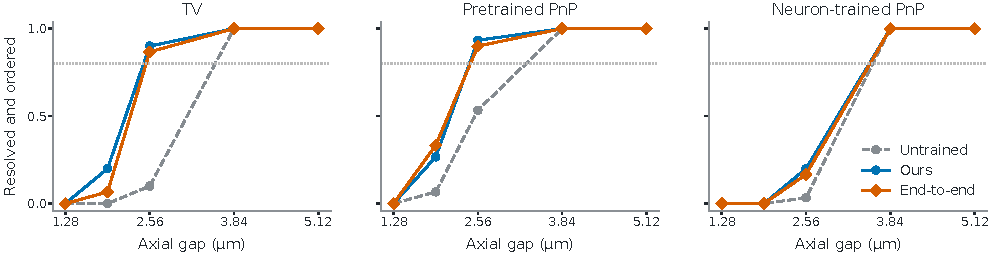
\includegraphics[width=\linewidth]{crossing_curves.pdf}
\caption{Full-dose equal-branch crossing curves for all three iterative methods, at $C=8$ and matched nominal dose. Each point pools three lateral geometries, two axial centers and five draws. The qualifying-gap rule requires at least 80\,\% success at each center separately and at all larger tested gaps. Under neuron-trained PnP, both the untrained and our plates qualify at $3.84\um$. Zero-gap controls have no false splitting.}
\label{fig:s:fullcrossings}
\end{figure*}

\paragraph{Merged neuronal alternatives.}
A reference column is called layered when it belongs to the signal mask and has at least two peaks under the same relative height/prominence rule. For each corresponding fine-grid lateral column, we move its intensity to its axial centroid, distributing mass between the two neighboring planes to preserve that centroid exactly. Other columns remain unchanged. The resulting alternative preserves the fine-grid lateral projection and each modified column's centroid while changing its depth profile. One crop has no eligible columns, leaving 59. These are constructed candidates, not solutions optimized over a measurement-consistency set; concentrated intensities need not remain below the original normalized peak.

For noise-free expected counts $\mu$ of the reference and $\nu(c)$ of a brightness-scaled alternative, we compute
\begin{equation}
D_{\mathrm P}(\mu\Vert\nu)=\sum_i\left[\mu_i\log\frac{\mu_i}{\nu_i}+\nu_i-\mu_i\right].
\end{equation}
The simulator evaluates both objects on the fine grid, using each matched direction subset and the same exposure. Without background, the profiled scale is the ratio of total reference to alternative expected counts. With background, the numerical fit searches a log-scale interval of $[-1,1]$ around the total-signal estimate. Crop scores average five subsets. The geometric mean of the crop-level learned/untrained ratios is 9.99 (95\,\% CI: 8.66--11.79) without background and 10.4 with background. Against the end-to-end plate, our ratio is 2.00 (1.91--2.09), with higher divergence on all 59 eligible crops. The draw-average is taken within each crop before forming the ratios. Untrained-plate divergences can already be large; the ratio is a diagnostic of these specified alternatives, not a probability of successful reconstruction. No KL-to-reconstruction-success guarantee is claimed.

\paragraph{Additional neuronal structure metrics.}
Layered columns carry about 17\,\% of reference signal on average. \Cref{tab:s:layered} uses the completed primary reconstruction rows and the 59 crops with eligible columns; one crop has none. Relative to the untrained plate, our plate lowers their profile W1 by 34\,\% with TV, 42\,\% with pretrained PnP and 28\,\% with neuron-trained PnP. The end-to-end plate has higher W1 than ours under TV, no established difference under either PnP method, and lower W1 with its own decoder. These descriptive subset results contextualize the single-column figures. Most eligible columns contain intensity structure within thick branches, so lower profile error does not establish separation of distinct neuronal branches or a larger benefit than in centroid accuracy.

A prespecified TV comparison did not establish a larger relative profile gain than centroid gain on layered columns: the difference was $-0.7$ percentage points (95\,\% CI: $-2.9$ to $+1.5$). PnP subset statistics remain descriptive because an earlier prespecified PSNR reproduction tolerance of $0.05$\,dB was not met; the completed full-field reruns use the numerical checks documented in \cref{sec:s:evaluation}.

\begin{table*}[t]
\centering\small
\widetab{\begin{tabular}{lrrrll}
\toprule
Reconstruction & Untrained & Ours & End-to-end & Ours vs. untrained & End-to-end minus ours \\
\midrule
TV & 0.467 & 0.309 & 0.318 & $-33.8\%$ [$-36.3$, $-31.7$] & $+0.009$ [$+0.004$, $+0.015$] \\
Pretrained PnP & 0.641 & 0.369 & 0.370 & $-42.4\%$ [$-46.5$, $-38.5$] & $+0.001$ [$-0.008$, $+0.009$] \\
Neuron-trained PnP & 0.374 & 0.271 & 0.272 & $-27.6\%$ [$-28.8$, $-26.4$] & $+0.001$ [$-0.002$, $+0.004$] \\
Feed-forward & 0.518 & 0.387 & 0.352 & $-25.4\%$ [$-29.6$, $-21.8$] & $-0.035$ [$-0.045$, $-0.028$] \\
\bottomrule
\end{tabular}
}
\caption{Profile W1 on layered reference columns: 59 eligible crops, $C=8$, five draws per crop, using the same completed reconstructions as the primary table. Errors and absolute end-to-end-minus-ours differences are in $\mu$m; brackets are paired cell-bootstrap 95\,\% intervals. Feed-forward decoders have the training histories in \cref{sec:s:joint}.}
\label{tab:s:layered}
\end{table*}

On all 60 crops, we also report centerline Dice \cite{shit2021}, which compares a reference mask at 10\,\% of peak intensity with an estimated mask retaining the same number of voxels, followed by 3D skeletonization. Scores rise from 0.79 to 0.84 for TV, 0.75 to 0.84 for pretrained PnP and 0.85 to 0.88 for neuron-trained PnP. This thresholded metric is depth-sensitive but does not substitute for branch tracing or connectivity validation.
